\section{Sample System Ouput - Units Data}
\begin{figure}[H]
	\centering
	\caption{accelX vs. Time}
		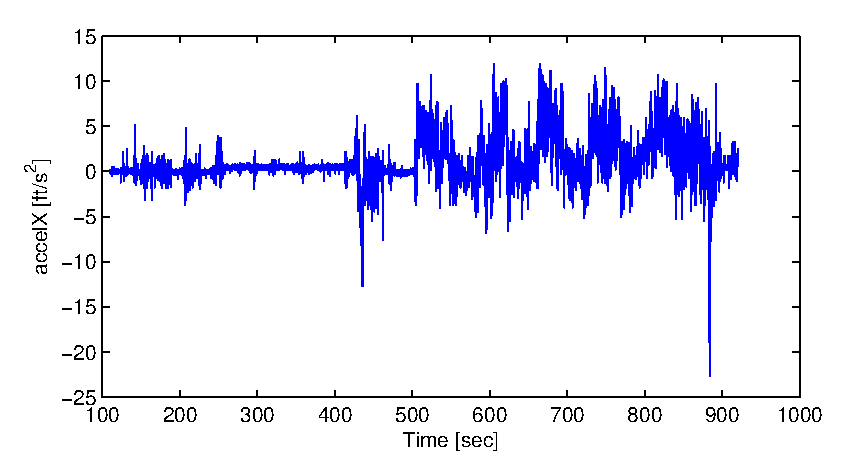
\includegraphics[width = 0.7\textwidth]{C:/Users/mufasa/Documents/Thesis/LaTex/figures/sampleOutput/Units/accelX.eps}
\end{figure}
\begin{figure}[H]
	\centering
	\caption{accelY vs. Time}
		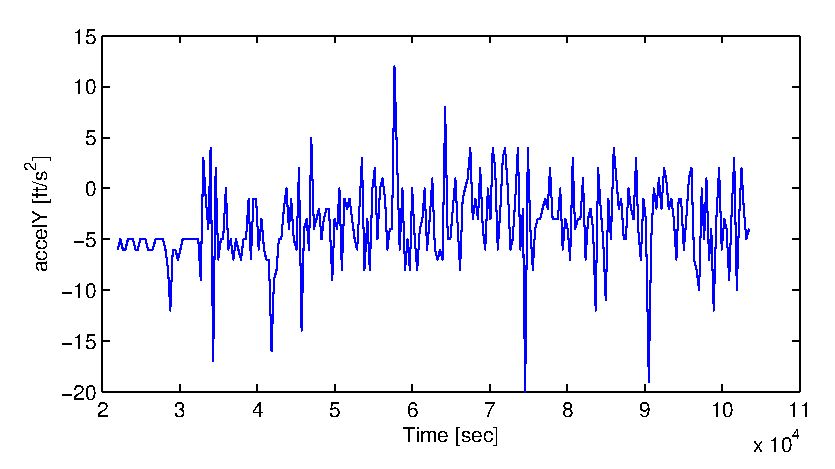
\includegraphics[width = 0.7\textwidth]{C:/Users/mufasa/Documents/Thesis/LaTex/figures/sampleOutput/Units/accelY.eps}
\end{figure}
\begin{figure}[H]
	\centering
	\caption{accelZ vs. Time}
		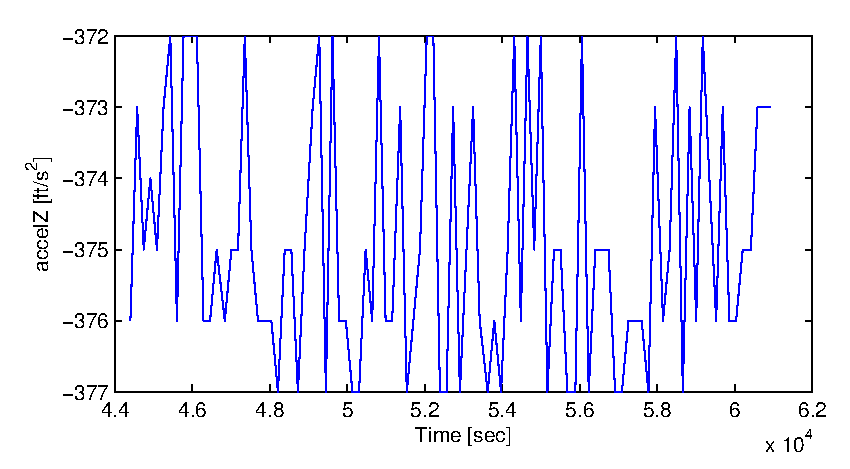
\includegraphics[width = 0.7\textwidth]{C:/Users/mufasa/Documents/Thesis/LaTex/figures/sampleOutput/Units/accelZ.eps}
\end{figure}
\begin{figure}[H]
	\centering
	\caption{gyroX vs. Time}
		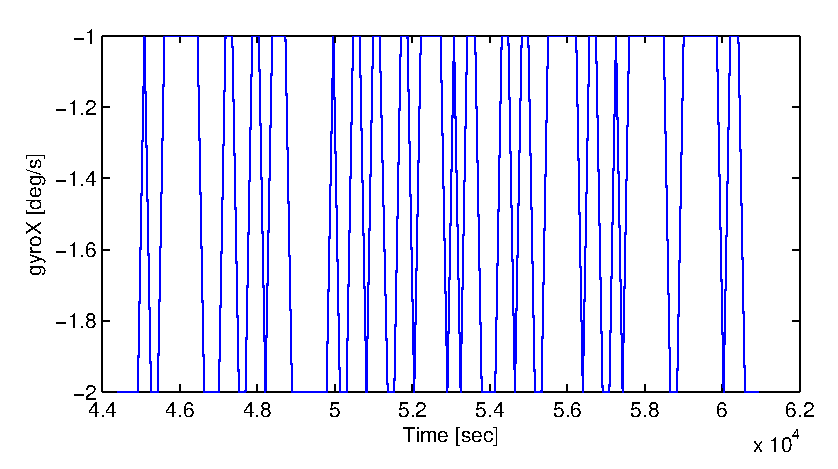
\includegraphics[width = 0.7\textwidth]{C:/Users/mufasa/Documents/Thesis/LaTex/figures/sampleOutput/Units/gyroX.eps}
\end{figure}
\begin{figure}[H]
	\centering
	\caption{gyroY vs. Time}
		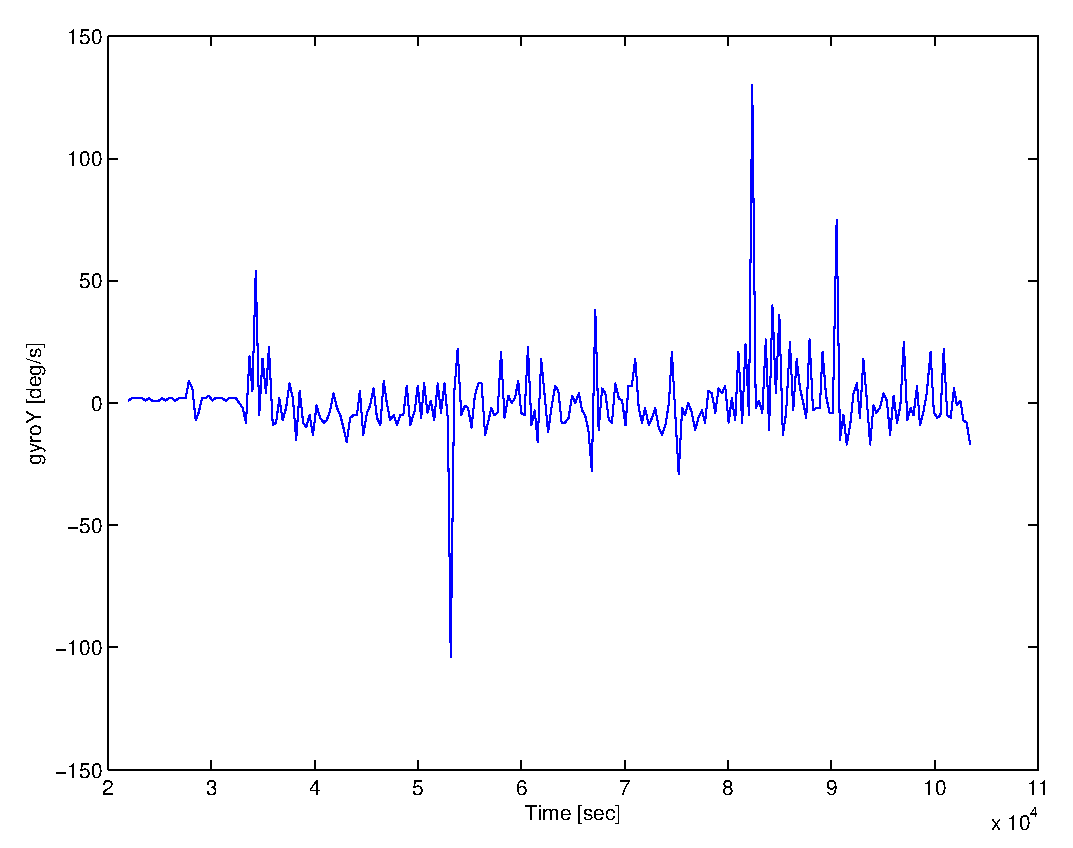
\includegraphics[width = 0.7\textwidth]{C:/Users/mufasa/Documents/Thesis/LaTex/figures/sampleOutput/Units/gyroY.eps}
\end{figure}
\begin{figure}[H]
	\centering
	\caption{gyroZ vs. Time}
		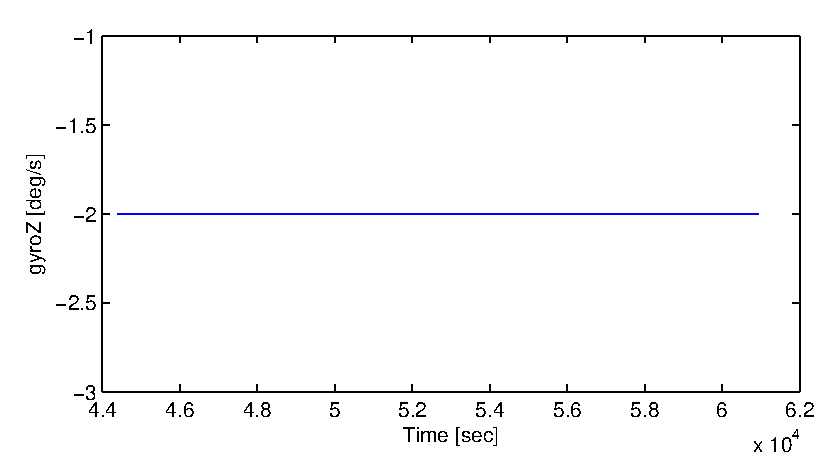
\includegraphics[width = 0.7\textwidth]{C:/Users/mufasa/Documents/Thesis/LaTex/figures/sampleOutput/Units/gyroZ.eps}
\end{figure}
\begin{figure}[H]
	\centering
	\caption{magX vs. Time}
		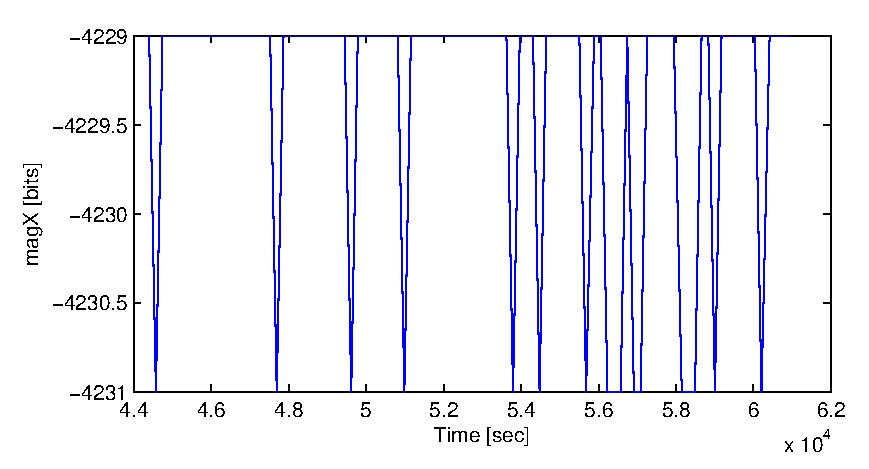
\includegraphics[width = 0.7\textwidth]{C:/Users/mufasa/Documents/Thesis/LaTex/figures/sampleOutput/Units/magX.eps}
\end{figure}
\clearpage
\begin{figure}[H]
	\centering
	\caption{magY vs. Time}
		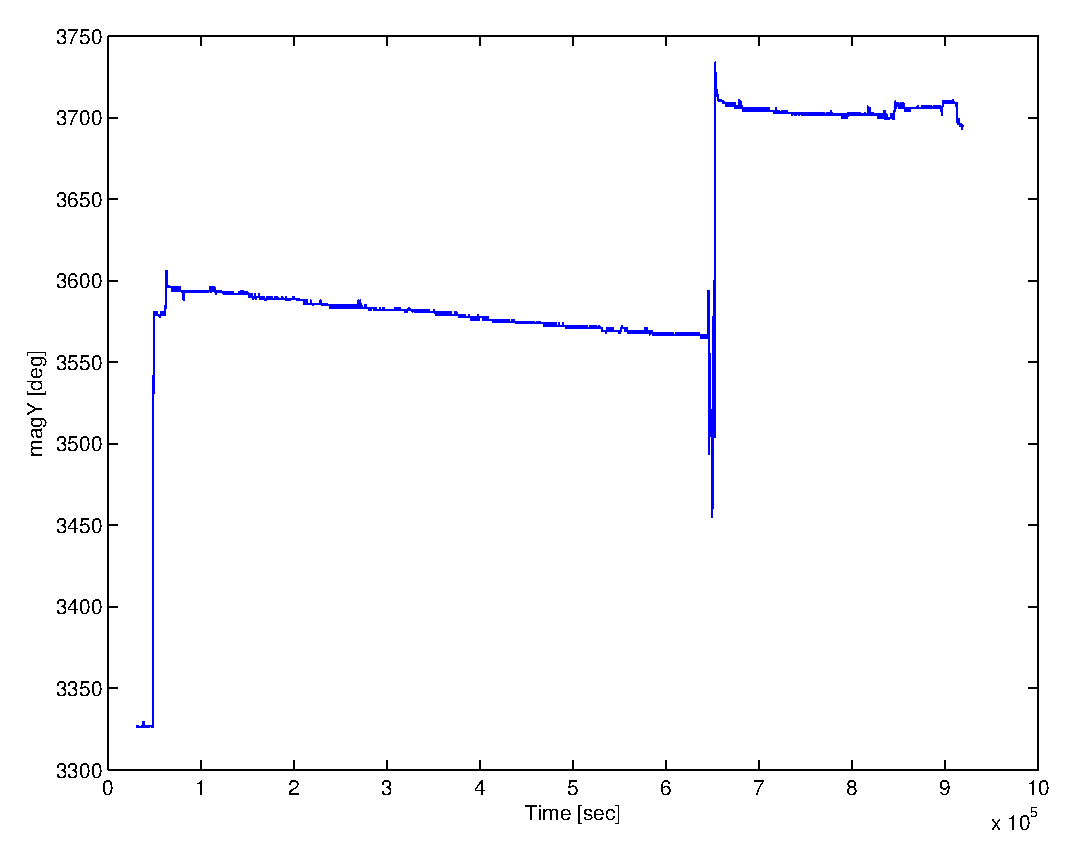
\includegraphics[width = 0.7\textwidth]{C:/Users/mufasa/Documents/Thesis/LaTex/figures/sampleOutput/Units/magY.eps}
\end{figure}
\begin{figure}[H]
	\centering
	\caption{magZ vs. Time}
		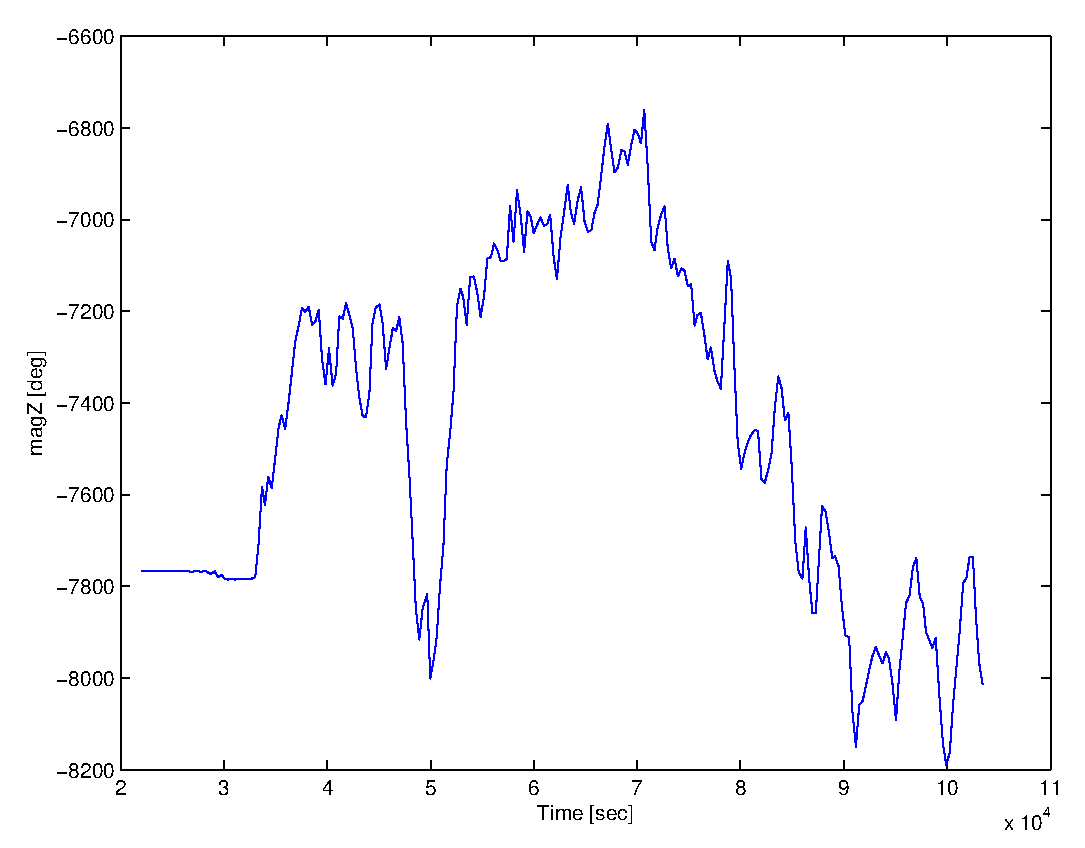
\includegraphics[width = 0.7\textwidth]{C:/Users/mufasa/Documents/Thesis/LaTex/figures/sampleOutput/Units/magZ.eps}
\end{figure}
\begin{figure}[H]
	\centering
	\caption{hmcX vs. Time}
		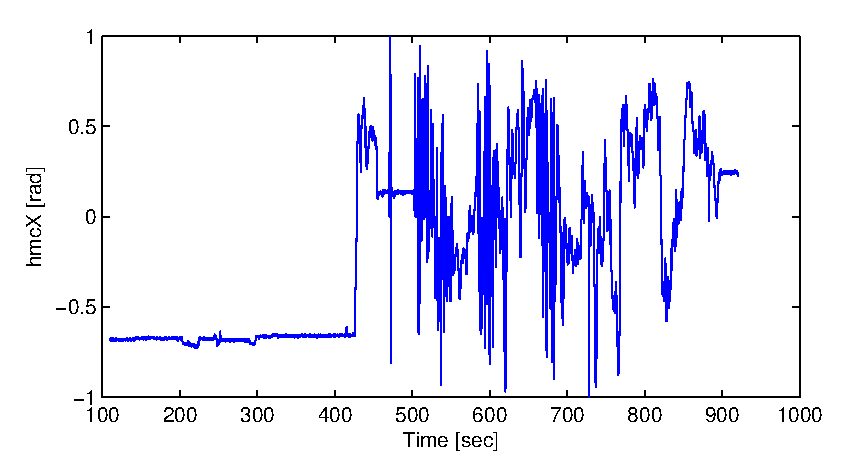
\includegraphics[width = 0.7\textwidth]{C:/Users/mufasa/Documents/Thesis/LaTex/figures/sampleOutput/Units/hmcX.eps}
\end{figure}
\begin{figure}[H]
	\centering
	\caption{hmcZ vs. Time}
		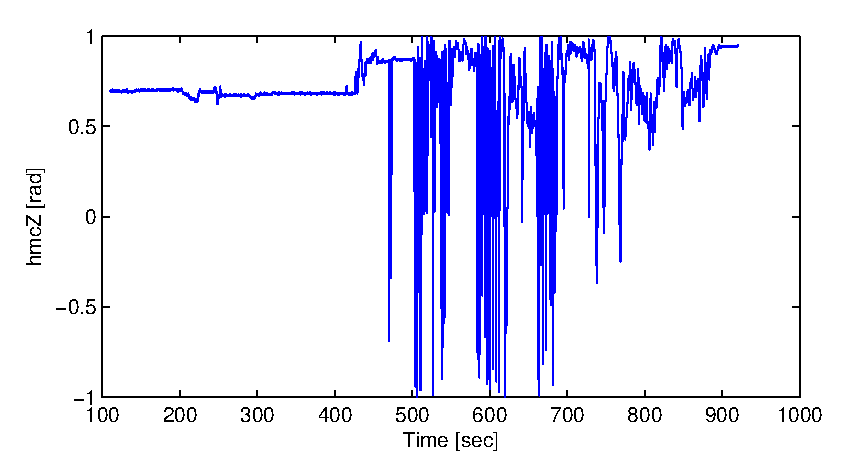
\includegraphics[width = 0.7\textwidth]{C:/Users/mufasa/Documents/Thesis/LaTex/figures/sampleOutput/Units/hmcZ.eps}
\end{figure}
\begin{figure}[H]
	\centering
	\caption{hmcY vs. Time}
		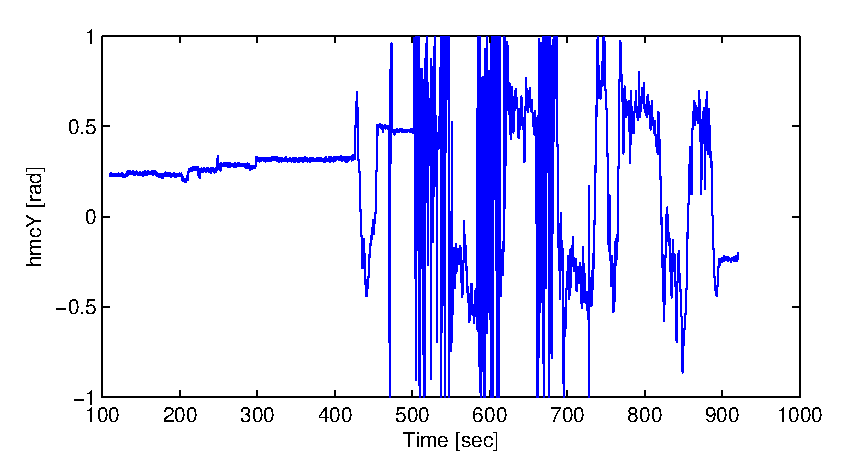
\includegraphics[width = 0.7\textwidth]{C:/Users/mufasa/Documents/Thesis/LaTex/figures/sampleOutput/Units/hmcY.eps}
\end{figure}
\begin{figure}[H]
	\centering
	\caption{press0 vs. Time}
		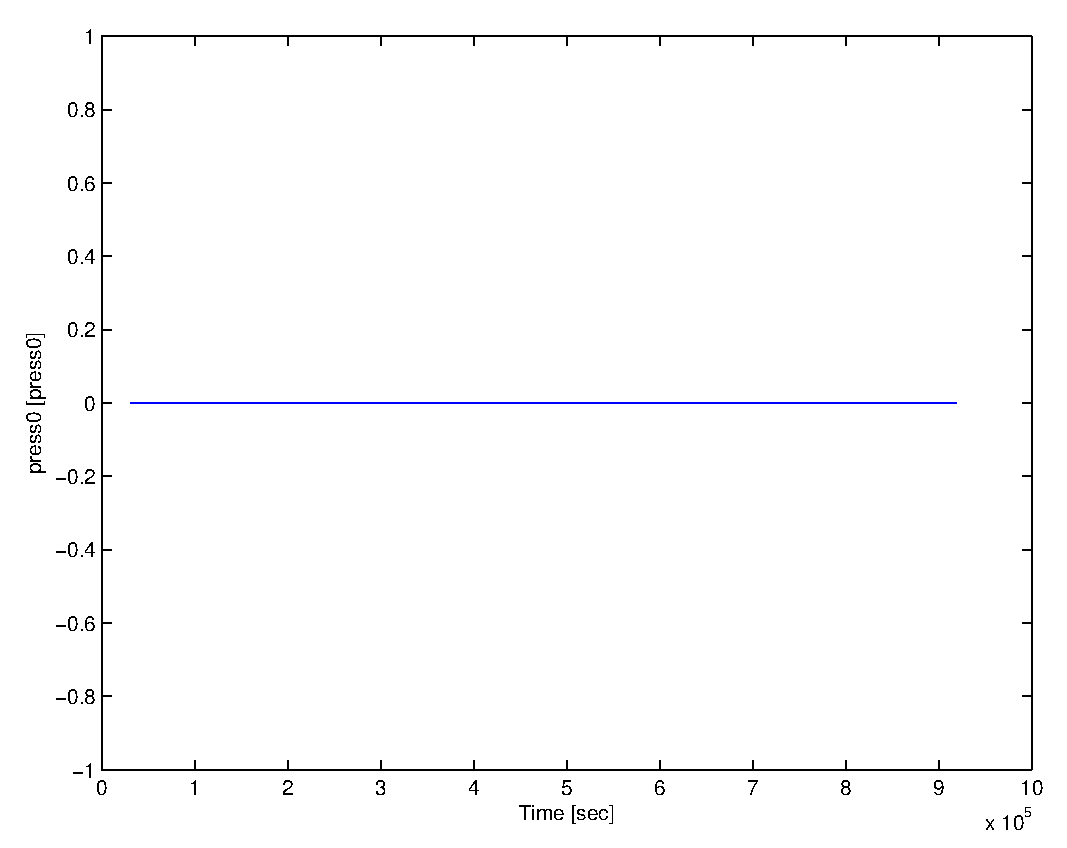
\includegraphics[width = 0.7\textwidth]{C:/Users/mufasa/Documents/Thesis/LaTex/figures/sampleOutput/Units/press0.eps}
\end{figure}
\begin{figure}[H]
	\centering
	\caption{press1 vs. Time}
		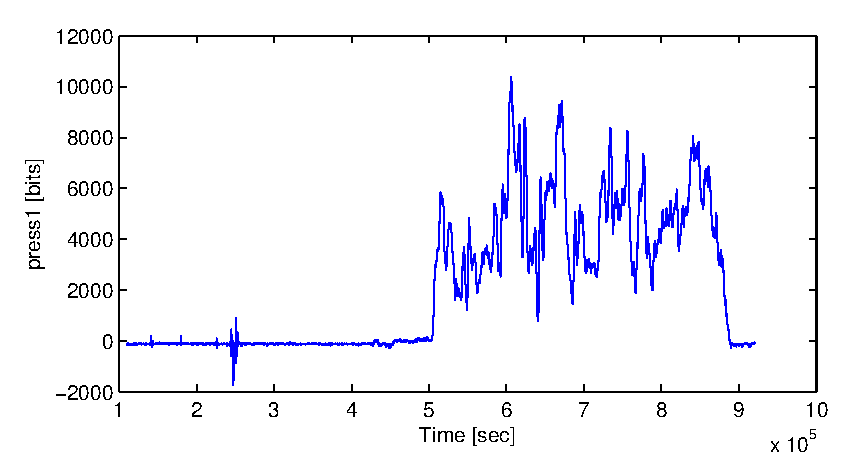
\includegraphics[width = 0.7\textwidth]{C:/Users/mufasa/Documents/Thesis/LaTex/figures/sampleOutput/Units/press1.eps}
\end{figure}
\begin{figure}[H]
	\centering
	\caption{press2 vs. Time}
		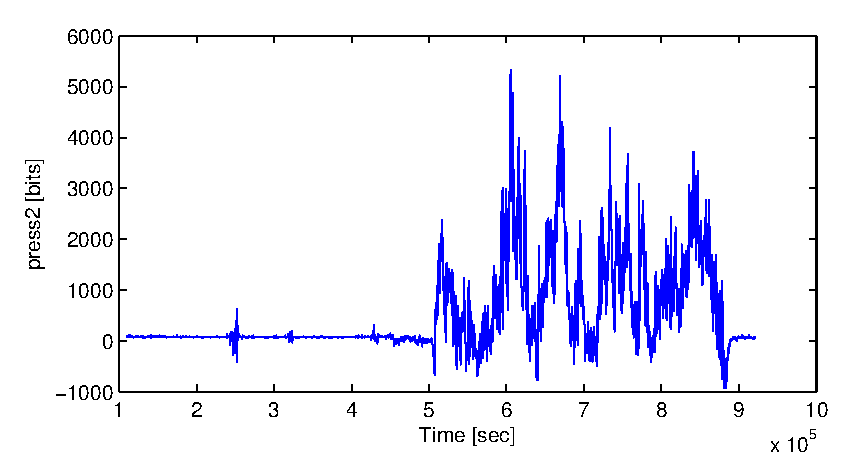
\includegraphics[width = 0.7\textwidth]{C:/Users/mufasa/Documents/Thesis/LaTex/figures/sampleOutput/Units/press2.eps}
\end{figure}
\begin{figure}[H]
	\centering
	\caption{press3 vs. Time}
		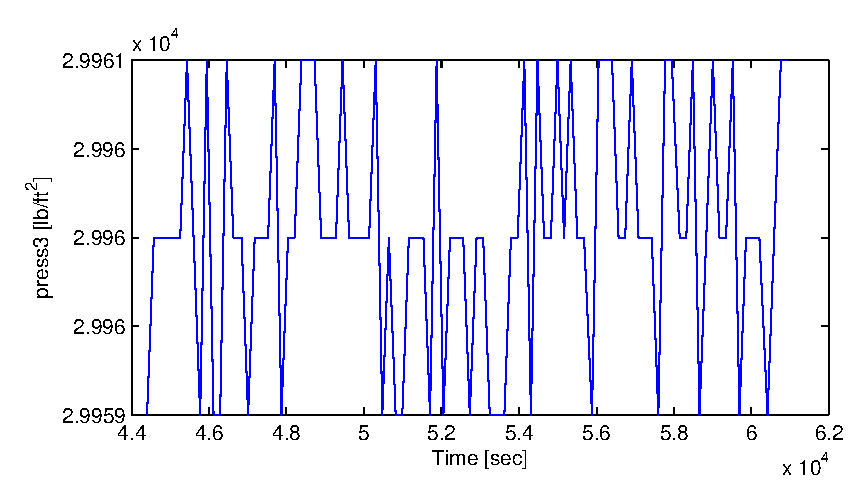
\includegraphics[width = 0.7\textwidth]{C:/Users/mufasa/Documents/Thesis/LaTex/figures/sampleOutput/Units/press3.eps}
\end{figure}
\begin{figure}[H]
	\centering
	\caption{gpsLat vs. Time}
		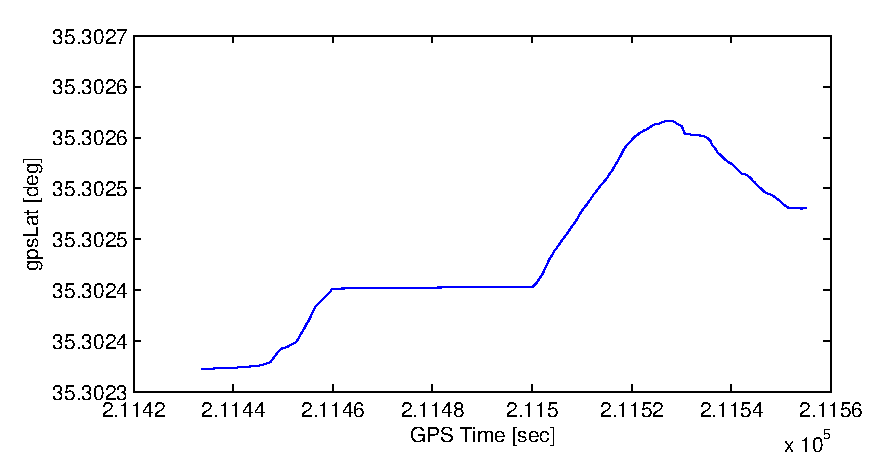
\includegraphics[width = 0.7\textwidth]{C:/Users/mufasa/Documents/Thesis/LaTex/figures/sampleOutput/Units/gpsLat.eps}
\end{figure}
\begin{figure}[H]
	\centering
	\caption{gpsLong vs. Time}
		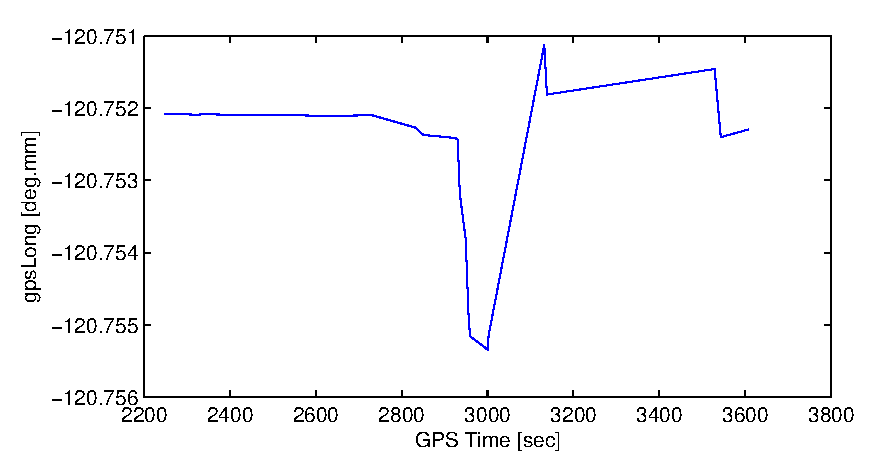
\includegraphics[width = 0.7\textwidth]{C:/Users/mufasa/Documents/Thesis/LaTex/figures/sampleOutput/Units/gpsLong.eps}
\end{figure}
\begin{figure}[H]
	\centering
	\caption{gpsSpd vs. Time}
		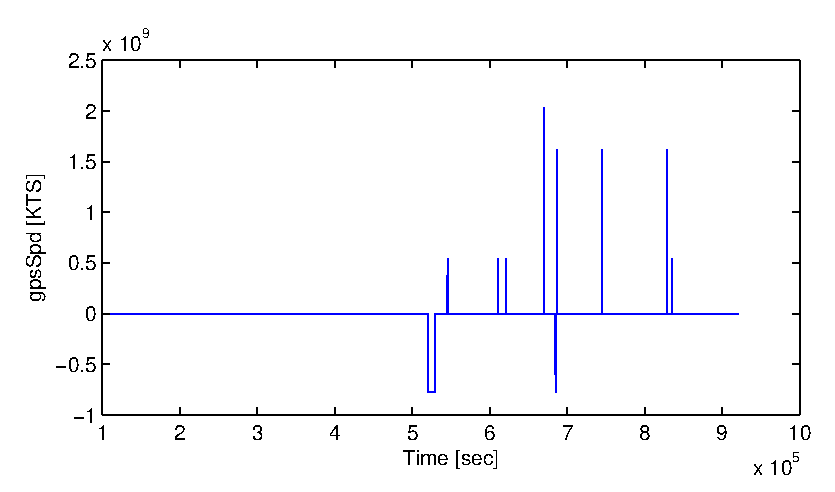
\includegraphics[width = 0.7\textwidth]{C:/Users/mufasa/Documents/Thesis/LaTex/figures/sampleOutput/Units/gpsSpd.eps}
\end{figure}
\begin{figure}[H]
	\centering
	\caption{gpsCrs vs. Time}
		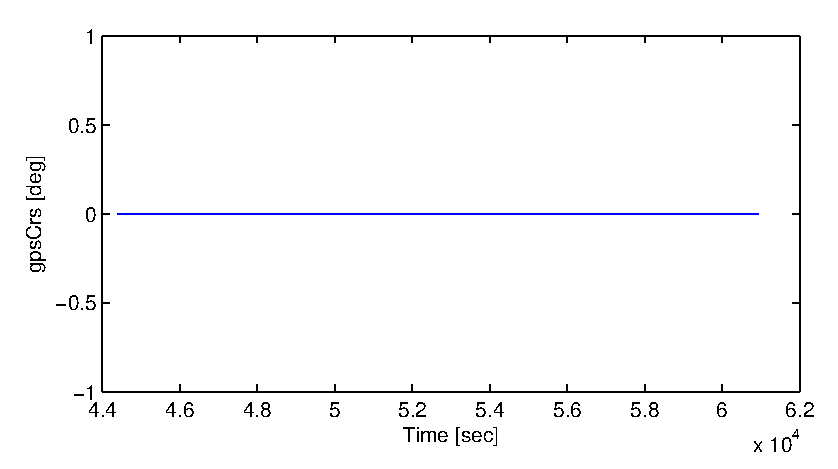
\includegraphics[width = 0.7\textwidth]{C:/Users/mufasa/Documents/Thesis/LaTex/figures/sampleOutput/Units/gpsCrs.eps}
\end{figure}
\begin{figure}[H]
	\centering
	\caption{date vs. Time}
		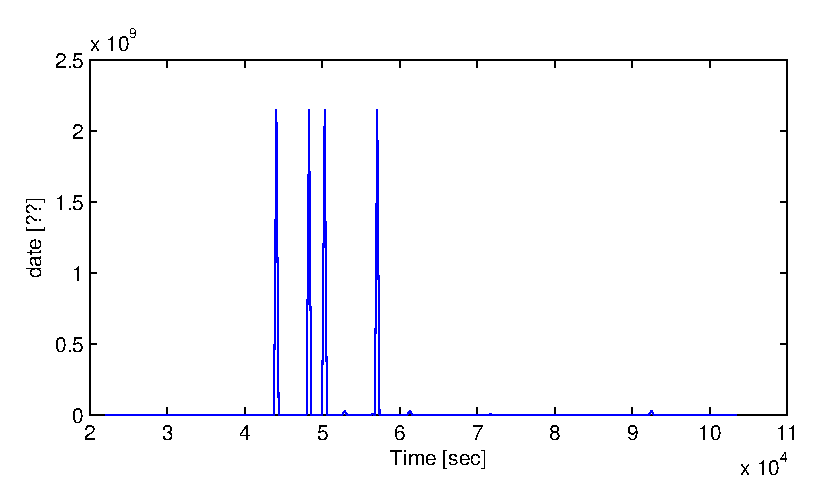
\includegraphics[width = 0.7\textwidth]{C:/Users/mufasa/Documents/Thesis/LaTex/figures/sampleOutput/Units/date.eps}
\end{figure}
\begin{figure}[H]
	\centering
	\caption{CS vs. Time}
		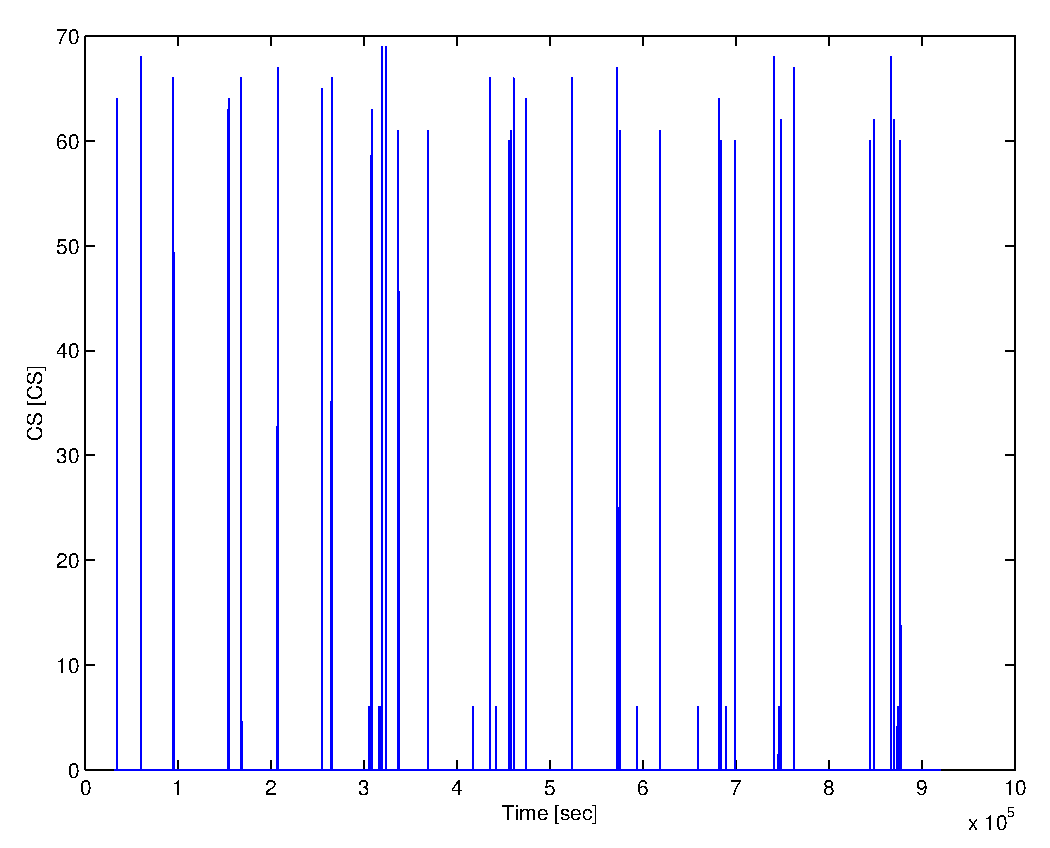
\includegraphics[width = 0.7\textwidth]{C:/Users/mufasa/Documents/Thesis/LaTex/figures/sampleOutput/Units/CS.eps}
\end{figure}
\begin{figure}[H]
	\centering
	\caption{temperature vs. Time}
		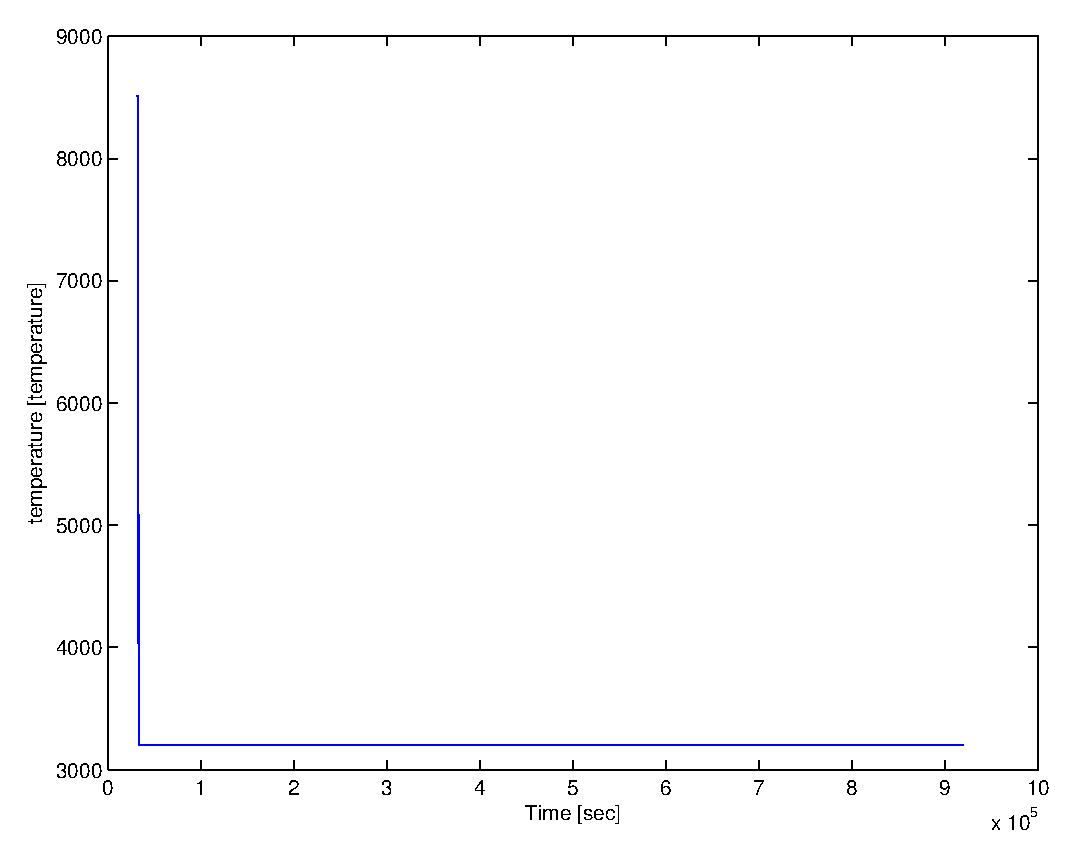
\includegraphics[width = 0.7\textwidth]{C:/Users/mufasa/Documents/Thesis/LaTex/figures/sampleOutput/Units/temperature.eps}
\end{figure}
\begin{figure}[H]
	\centering
	\caption{pwm0 vs. Time}
		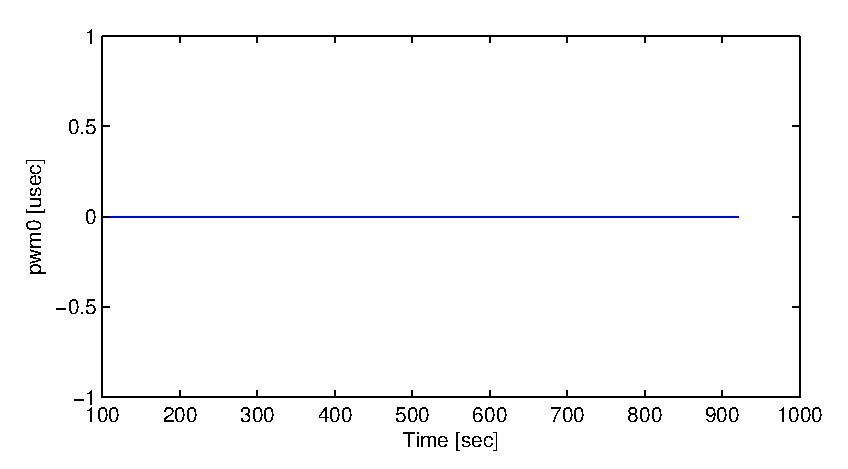
\includegraphics[width = 0.7\textwidth]{C:/Users/mufasa/Documents/Thesis/LaTex/figures/sampleOutput/Units/pwm0.eps}
\end{figure}
\begin{figure}[H]
	\centering
	\caption{pwm1 vs. Time}
		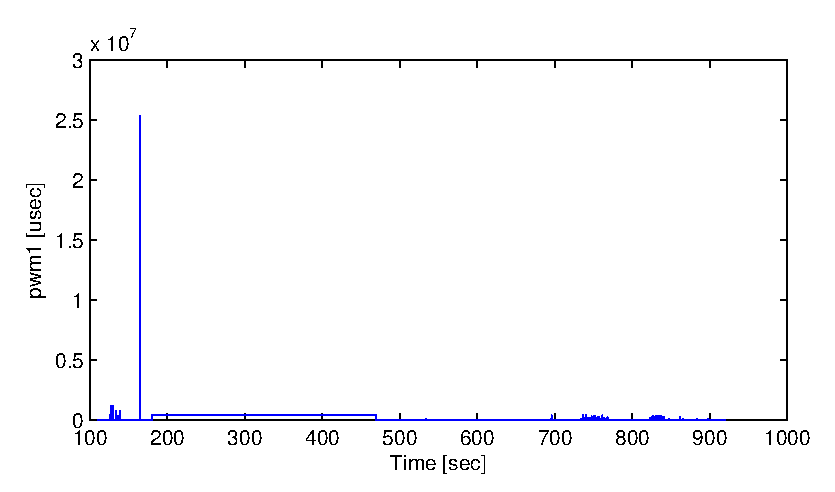
\includegraphics[width = 0.7\textwidth]{C:/Users/mufasa/Documents/Thesis/LaTex/figures/sampleOutput/Units/pwm1.eps}
\end{figure}
\begin{figure}[H]
	\centering
	\caption{pwm2 vs. Time}
		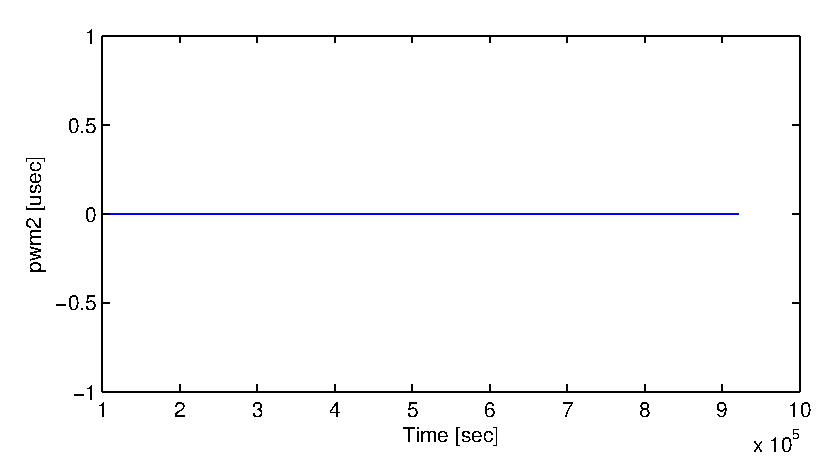
\includegraphics[width = 0.7\textwidth]{C:/Users/mufasa/Documents/Thesis/LaTex/figures/sampleOutput/Units/pwm2.eps}
\end{figure}
\begin{figure}[H]
	\centering
	\caption{pwm3 vs. Time}
		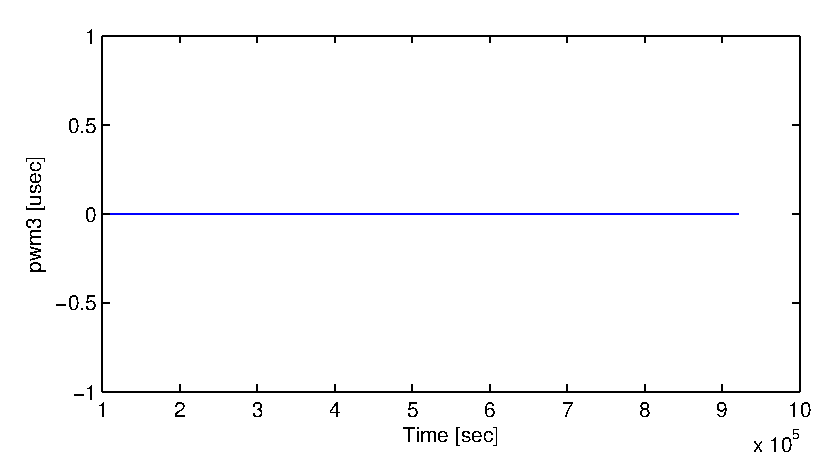
\includegraphics[width = 0.7\textwidth]{C:/Users/mufasa/Documents/Thesis/LaTex/figures/sampleOutput/Units/pwm3.eps}
\end{figure}
\begin{figure}[H]
	\centering
	\caption{pwm4 vs. Time}
		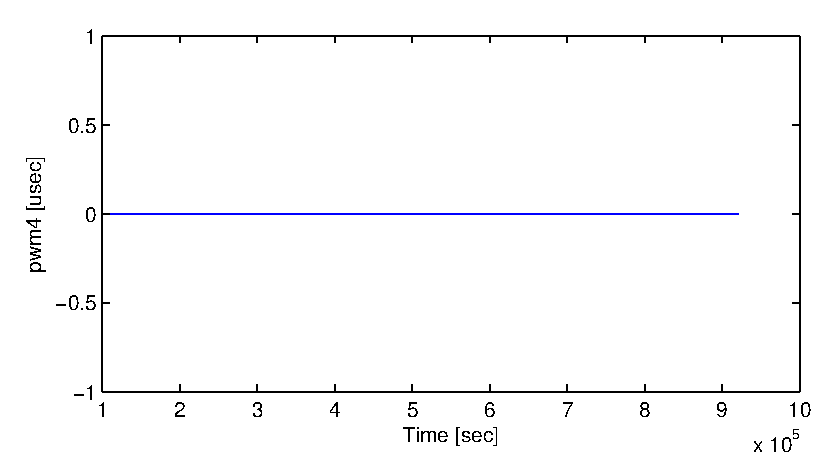
\includegraphics[width = 0.7\textwidth]{C:/Users/mufasa/Documents/Thesis/LaTex/figures/sampleOutput/Units/pwm4.eps}
\end{figure}
\begin{figure}[H]
	\centering
	\caption{pwm5 vs. Time}
		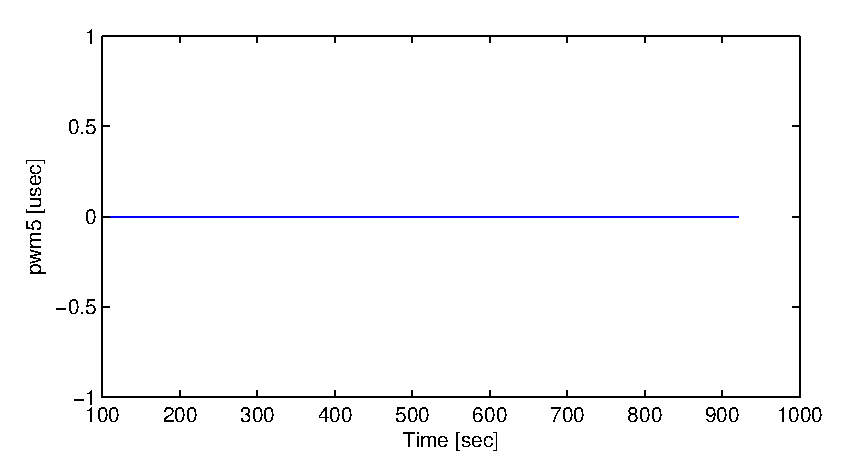
\includegraphics[width = 0.7\textwidth]{C:/Users/mufasa/Documents/Thesis/LaTex/figures/sampleOutput/Units/pwm5.eps}
\end{figure}
\begin{figure}[H]
	\centering
	\caption{pwm6 vs. Time}
		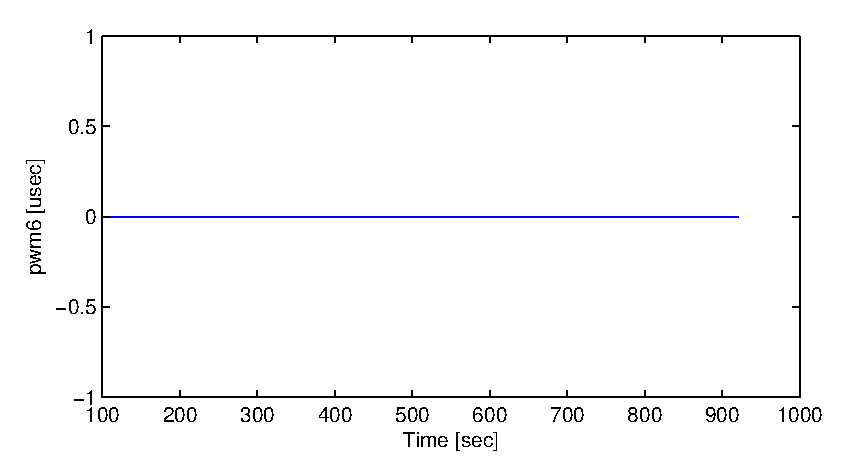
\includegraphics[width = 0.7\textwidth]{C:/Users/mufasa/Documents/Thesis/LaTex/figures/sampleOutput/Units/pwm6.eps}
\end{figure}
\begin{figure}[H]
	\centering
	\caption{pwm7 vs. Time}
		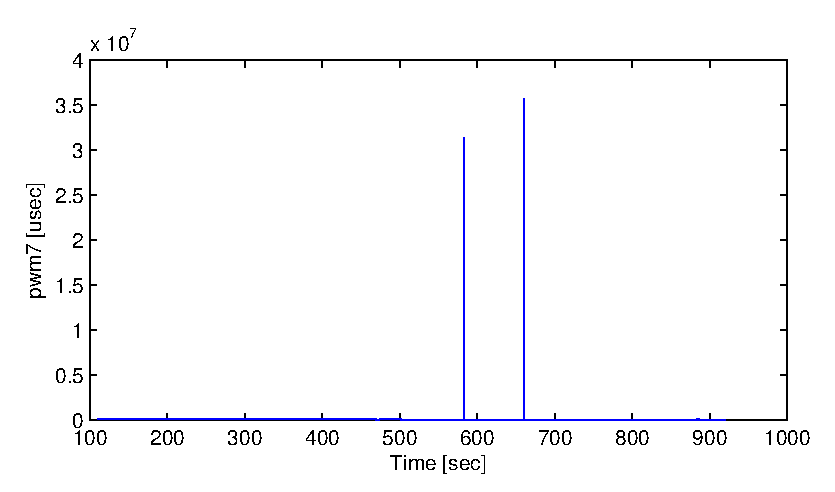
\includegraphics[width = 0.7\textwidth]{C:/Users/mufasa/Documents/Thesis/LaTex/figures/sampleOutput/Units/pwm7.eps}
\end{figure}
\begin{figure}[H]
	\centering
	\caption{deltaT vs. Time}
		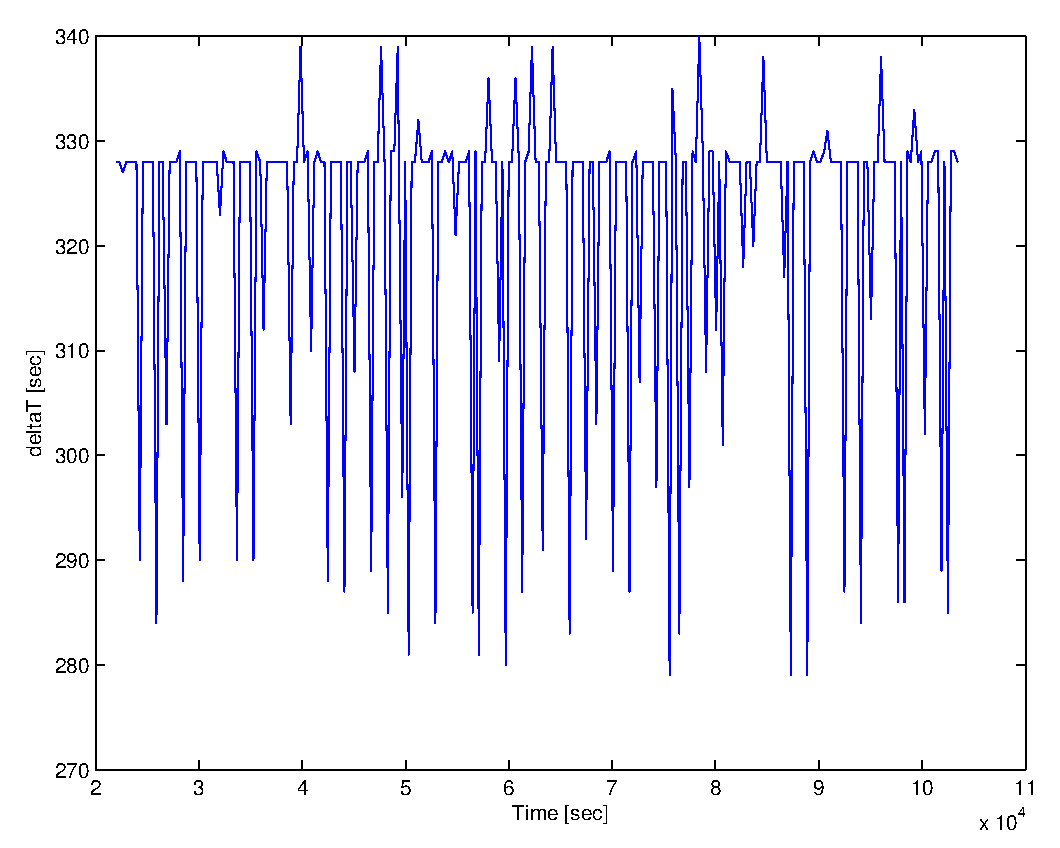
\includegraphics[width = 0.7\textwidth]{C:/Users/mufasa/Documents/Thesis/LaTex/figures/sampleOutput/Units/deltaT.eps}
\end{figure}
